\documentclass[a4paper, 12pt]{article}
\usepackage[slovene]{babel}
\usepackage[utf8]{inputenc}
\usepackage[T1]{fontenc}

\usepackage{amsmath, amssymb, hyperref, fullpage, float, caption}
\usepackage[usenames, dvipsnames]{xcolor}
\usepackage[pdftex]{graphicx}

%to get the colourful hyperlinks ... not just square boxes around them ...
\hypersetup{
	colorlinks=true,
	linkcolor=black!60!red,
	citecolor=black!60!green,
	urlcolor=black!60!cyan,
	filecolor=black!60!magenta
}

%set up custom captions
\captionsetup{
	font=small,
	margin=10pt,
	labelfont=it,
	format=hang,
	width=0.9\textwidth
}

\newcommand{\px}{
	\ensuremath{\partial_x}
}

\newcommand{\pt}{
	\ensuremath{\partial_t}
}

\renewcommand{\H}{
	\ensuremath{\mathbf{H}}
}

\newcommand{\I}{
	\ensuremath{\mathbf{I}}
}

\newcommand{\Tr}{
	\operatorname{Tr}
}

\newcommand{\e}{
	\ensuremath{\text{e}}
}

\newcommand{\cosec}{
	\operatorname{cosec}
}

\newcommand{\pr}{
	\ensuremath{\underline{p}}
}

\newcommand{\w}{
	\ensuremath{\omega}
}

\renewcommand{\d}{
	\ensuremath{\text{d}}
}

\newcommand{\odv}[1][{}\ ]{
	\ensuremath{\frac{\d^#1}{\d x^#1}}
}

\renewenvironment{abstract}[1][1.0]
{
	\begin{center}
		{\bf Povzetek}\\[12pt]
		\begin{minipage}{#1\textwidth}
}
{
		\end{minipage}
	\end{center}
}

\newcommand{\koren}{
	\ensuremath{\frac{1}{\sqrt{2}}}
}

\newcommand{\intinf}{
	\ensuremath{\int_{-\infty}^\infty\d x}
}

\newcommand{\pe}{
	\ensuremath{\partial_\eta}
}

\renewcommand{\ni}{
	\noindent
}

\begin{document}

% titlepage
\begin{titlepage}
	\begin{figure}[H]
		\centering
		
\includegraphics[width = 7cm, keepaspectratio=1]{pics/logo.pdf}\\[12pt]
		{\sc Oddelek za fiziko}\\[4cm]
	\end{figure}
	\begin{center}
		\large{Seminar -- 1. letnik fizike, druge bolonjske stopnje}\\[0.5cm]
		\LARGE\textbf{Supersimetrija v klasi\v cni kvantni mehaniki}\\[1.0cm]

		\vspace{0.0cm}

		\begin{minipage}{0.4\textwidth}\small
			\begin{flushleft}
			\textsc{Avtor:}\\[0.2cm]
			Jo\v ze Zobec, dipl. fiz. (UN)
			\end{flushleft}
		\end{minipage}
		\begin{minipage}{0.4\textwidth}\small
			\begin{flushright}
				\textsc{Mentor:}\\[0.2cm]
				Prof. Dr. Svjetlana Fajfer,\\[0.1cm]
				Prof. Dr. Toma\v z Prosen
			\end{flushright}
		\end{minipage}
	\end{center}

	\vspace{5.0cm}

	\begin{abstract}
		Supersimetrija je \v sir\v se podro\v cje, ki ni omejeno zgolj na fiziko osnovnih
		delcev, pa\v c pa na celotno kvantni mehaniko. V tem seminarju bom pokazal
		ra\v cunske prijeme v obravnavi klasi\v cnih kvantno-mehanskih problemih s pomo\v cjo
		supersimetri\v cnega ogrodja in novosti v teoriji izospektralnih Hamiltonianov ter
		teoriji perturbacij.
	\end{abstract}
	
	\vfill

	\centering{\footnotesize Ljubljana, \today}
\end{titlepage}



\tableofcontents

\pagebreak

\chapter{Uvod}

Standardni model je ta hip najbolj precizna teorija v fiziki. Delce, za katere ta hip empirično
verjamemo, da so nedeljivi, smiselno razvrsti in opiše njihove interakcije ter tako pojasni
makroskopske pojave s pomočjo najosnovnejših pojavov, ki se dogajajo na zelo majhni skali.

Kljub dobrim in zelo lepin lastnostim standardnega modela, obstajajo eksperimentalne indikacije, da
standardni model ni popoln. S teoretičnega vidika bi zelo težko pojasnili izmerjeno asimetrijo $CP$
in pa nesorazmernost v vsebnosti snovi proti vsebnosti anti-snovi v našem vesolju. To bi lahko pojasnili
z razpadom protona, ki ni dovoljen v standardnem modelu. Prav tako zahteva zahteva, da so nevtrini
brezmasni, ni več podprta s strani eksperimentov, a standardni model jih ne more umestiti drugače.
Še ena hiba standardnega modela je ta, da ne more pojasniti kvantizacije električnega naboja in ne more
predvideti števila generacij fermionov.

Standardni model med fermionskimi polji opisuje tri fundamentalne interakcije in njihove nosilce, ki so
bozoni. Te tri interakcije so močna, šibka in elektromagnetna. Ker so osnovni delci izjemno lahki,
gravitacijo zanemarimo, ta bi sicer bila četrta fundamentalna interakcija. Kako naj torej pojasnimo
npr. razpad protona? Lahko ugibamo o obstoju nove, še neodkrite interakcije, katere vloga postane
bolj očitna pri višjih energijah. Poleg bozonov, ki so nosilci interakcij obstajajo tudi ti. Higgsovi
bozoni, ki dajo maso prek Higgsovega mehanizma, na račun tega, da interakcijo zadušijo na nizkih
energijskih skalah.  Tako bi lahko dali nevtrinom mase in omogočili protonski razpad.

Tak način razmišljanja je odprl novo raziskovalno področje v teoriji osnovnih delcev, ki se imenuje
teorija poenotenja\footnote{\emph{ang.} Grand Unified Theory -- GUT.}, ki skuša iti korak dlje -- namesto
tega, da bi dodali le eno novo interakcijo, trdimo da v osnovi obstaja le ena sama, ki se zaradi
prisotnosti Higgsovih polj prikazuje v treh oblikah. Tak pristop nam omogoča poenostavitev, saj poleg
poenotenja znanih interakcij, poenotimo tudi fermionska polja. S seboj pa prinese tudi komplikacije,
saj ima tipično več nosilcev interakcij -- te uporabimo za teoretično pojasnilo eksperimentov, ki se
jih ni dalo znotraj standardnega modela. S pravo teorijo poenotenja bi lahko pojasnili vse to, kar
nam manjka.

Na žalost, pa je tako teorijo zelo težko preveriti. Poenotenje se predvidoma zgodi na energijski skali
$\Lambda_\text{GUT} \approx 2 \cdot 10^{16}$ GeV~\cite{mohapatra}. Zaenkrat smo z eksperimenti šele
pričeli z raziskovanjem področja od $100$ GeV do $1000$ GeV kar je zaenkrat inženirski podvig znanih
prijemov. Obstaja realna možnost, da ne bomo nikdar mogli potrditi oz. ovreči teorije poenotenja.

Vendar, če bomo opazili protonski razpad, bomo zmožni prav tega. In ne le to -- prek študije
protonskega razpada bomo mogli tudi povedati katera interakcija je tista v visokih energijah, tj. s
katero umeritveno grupo jo lahko opišemo. To je možno narediti z eksperimenti pri nizkih energijah,
ki se odvijajo na Japonskem, v Super-Kamiokande. Odsotnost protonskega razpada pa žal teorije poenotenja
ne more ovreči, saj so obstajajo tako teorije, ki ga vsebujejo, kot tudi, ki ga nimajo.

V teoriji poenotenja so glavni kandidati za umeritveno grupo poenotene interakcije predvsem $SU(5)$,
$SO(10)$ in $E_6$. Prva teorija poenotenja je bila narejena ravno prek $SU(5)$, katera pa ima še vedno
sterilne desnoročne nevtrine, ki bi jih potrebovali za maso. Pričakujemo, da tudi slednji sodelujejo
v interakcijah. To lahko storimo z umeritveno grupo $SO(10)$, ki pa nam da pravo bogastvo. Poleg tega,
da kvantizira električni naboj, je to tudi teorija "`levo-desno"' simetričnega vesolja. Pri nizkih
energijah imajo namreč ti. levoročni delci poseben status. Še vedno pa to ni teorija, ki bi napovedala
število generacij -- za to bi potrebovali vsaj $SU(9)$, ki ima za podgrupo
$SU(3)_L\times SU(3)_C\times U(1)_X$, kot so to storili v \cite{SU9}.

Tudi mi bomo tekom tega dela uporabili model poenotenja prek $SO(10)$. Osredotočili se bomo predvsem
na problem nevtrinskih mas in mešalne matrike v leptonskem sektorju, to je matrike
Pontecorvo-Maki-Nakagawa-Sakata (PMNS), ki je analogija mešalne matrike v kvarkovskem sektorju,
Cabbibo-Kobayashi-Maskawa (CKM).

To delo je v grobem razdeljeno na tri dele. V prvem delu bomo na kratko povzeli standardni model,
teorijo poenotenja $SO(10)$ in mehanizem, ki da nevtrinom mase. V drugem delu bomo predstavili
teoretičen model, ki ga bomo preučili tekom tega dela. Tretji del bo namenjen diskusiji rezultatov.
Delali bomo v enotah $\hbar = c = \varepsilon_0 = 1$.


\section{Ponovitev}

Iz predavanj Vi\v sje kvantne mehanike se spomnimo, da lahko polja
kvantiziramo prek operatorjev polja, za kar pa nujno potrebujemo kreacijske, $a^\dagger$ in 
anihilacijske $a$ operatorje. Na kratko ponovimo nekaj pojmov, s katerimi se bomo sre\v cevali tekom tega
seminarja.

\subsection{Grupa}

\vspace{0.5 cm}

{\em Grupa} je mno\v zica elementov z naslednjimi lastnostmi:

\begin{enumerate}
	\item{Med elementi obstaja asociativna operacija.}
	\item{Mno\v zica je za to operacijo zaprta.}
	\item{Izmed teh elementov je natanko eden tak, ki je za to operacijo enota.}
	\item{V mno\v zici so zajeti tudi vsi inverzni elementi.}
\end{enumerate}

V kolikor ne veljajo vsi pogoji imamo enega izmed ni\v zjih objektov, kot je na primer monoid (nimamo
nujno vseh inverzov) ali polgrupa (nimamo nujno udentitete).

\v Ce je operacija komutativna, je ta grupa abelova in operacijo imenujemo se\v stevanje. Sicer
pa je grupa neabelova in operacijo imenujemo mno\v zenje.

\subsection{Algebra}

\vspace{0.5cm}

Pogostokrat sre\v camo pojem `algebra'. Pa ponovimo, kaj je to.\\

\emph{Kolobar} je mno\v zica elementov z naslednjimi lastnostmi:

\begin{enumerate}
	\item{Ta mno\v zica je abelova grupa z operacijo se\v stevanja.}
	\item{Elementi so hkrati (pol)grupa za operacijo mno\v zenja.}
	\item{Za kombinacijo operacij velja distributivnostna relacija.}
\end{enumerate}

\emph{Algebra} je vektorski prostor nad kolobarjem.

Liejeve grupe imajo tudi svojo algebro -- generatorji Liejevih grup nepenjajo vektorski
prostor na mnogoterosti grupe\footnote{Vsaka Liejeva grupa je hkrati mnogoterost}. Da poka\v zemo,
da zado\v s\v cajo pogojem iz algebre zado\v s\v ca zapis komutacijskih relacij med generatorji, zato
bomo na tem mestu definirali komutator, en.~\eqref{komutator} in anti-komutator, en.~\eqref{antikomutator}:

\begin{align}
	[A,B] &\equiv AB - BA, \label{komutator}\\
	\{A,B\} &\equiv AB + BA. \label{antikomutator}
\end{align}

Vpeljali bomo skupno notacijo, s katero bomo lahko "`me\v sali"' med obema pojmoma:

\begin{align}
	[A,B]_\pm = AB \pm BA.
\end{align}

Tudi kon\v cnim grupam lahko priredimo algebre -- za nas relevantna je simetri\v cna grupa
$S_n$, ki jo imenujemo tudi permutacijska grupa.

\v Ce to grupo raz\v sirimo z operacijo parnosti, ima ta nova grupa dve nerazcepni upodobitvi. Funkcije so lahko
bodisi simetri\v cne na permutacije, ali pa anti-simetri\v cne. Baza za prvo upodobitev so bozonski, za drugo
pa fermionski kreacijsko-anihilacijski operatorji.

Lastne vrednosti so $\pm 1$ (parnost), hkrati pa grupa komutira s Hamiltonianom, kar pomeni,
da je to dobra simetrija in da Hamiltonian lahko zapi\v semo tako, v bazi te upodobitve, oz. druga\v ce:
Hamiltonian lahko zapi\v semo s pomo\v cjo fermionskih ali bozonskih kreacijsko-anihilaijckih operatorjev.

Tako od tu dobimo fermionsko in bozonsko algebro:

\begin{align}
	[a_i, a_j^\dagger]_\pm &= \delta_{ij}, \\
	[a_i, a_j]_\pm &= 0,
\end{align}

kjer komutatorji ustrezajo bozonom, antikomutatorji pa fermionom.

\section{Uvod v supersimetrijo}

Pa si omo\v cimo noge v vodi supersimetrije: obravnavajmo Schr\" odingerjevo ena\v cbo, tj. Hamiltonian

\begin{equation}
	H = -\frac{\hbar^2}{2m}\nabla^2 + mV(\vec{x}).
	\label{schroedinger}
\end{equation}

Vpeljemo enote $\hbar = c_0 = \varepsilon_0 = 1$. Maso $m$ bomo zaenkrat postavili na $1$. Tako je brezdimenzijska
Schr\" odingerjeva ena\v cba

\begin{equation}
	H = -\frac{1}{2}\nabla^2 + V(\vec{x}),
	\label{s1}
\end{equation}

kjer velja \v se $H = i\pt$. V eni dimenziji se~\eqref{s1} glasi

\begin{equation}
	H = -\frac{1}{2}\px^2 + V(x).
	\label{sx}
\end{equation}

Predpostavimo, da je na\v s potencial neni\v celen in navzdol omejen.

Velja

\begin{equation}
	H\psi_n(x) = E_n\psi_n(x) = i\pt\psi_n(x).
\end{equation}

Za $E_0 = 0$ torej velja $H|\psi_0\rangle = 0$. Od tu dobimo pogoj za potencial

\begin{equation}
	V(x) = \frac{1}{2}\frac{\px^2\psi_0}{\psi_0},
	\label{vpogoj}
\end{equation}

kjer smo predpostavili, da so stanja $\psi_n(x)$ vezana stanja, tj. je $\psi_0(x)$ dobro dolo\v cen, in
to lahko storimo.

Na\v s Hamiltonian bi radi zapisali v obliko z operatorjem \v stetja, $a^\dagger$ in $a$, se pravi
$H = a^\dagger a$, zato moramo poiskati nek pameten razcep. Vidimo, da je~\eqref{sx} oblike
$H \sim (A + B)(A - B)$, tako bomo definirali superpotencial $W(x)$, da bo

\begin{align}
	a &= W(x) + \frac{1}{\sqrt{2}}\px, \\
	a^\dagger &= W(x) - \frac{1}{\sqrt{2}}\px.
\end{align}

Taka operatorja sta res drug drugemu hermitsko adjungirana, saj je operator $\px$ anti-hermitski (do totalnega
odvoda natan\v cno).

Vse lepo in prav, vendar, a tak $W (x)$ sploh obstaja? V fiziki na taka vpra\v sanja ponavadi odgovorimo
retrospektivno in to bomo storili tudi sedaj. Vse skupaj vstavimo v Hamiltonian in iz njega dolo\v cimo
vezi, katerim mora zado\v s\v cati.

Poglejmo, kaj naredi $a^\dagger a$ na neki funkciji $\phi (x)$:

\begin{align}
	a^\dagger a\ \phi(x)&= \Big[W(x) - \frac{1}{\sqrt{2}}\px\Big]\Big[W(x) +
		\frac{1}{\sqrt{2}}\px\Big]\phi(x) \notag \\
	&= \Big[-\frac{1}{2}\px^2 + W^2(x)\Big]\phi(x) - \frac{1}{\sqrt{2}}\Big[
		\underbrace{\px \big(W(x)\phi(x)\big) - W(x)\px\phi(x)}_{(\px W(x))\phi(x)} \Big] \notag \\
	&= \bigg\{-\frac{1}{2}\px^2 +
		\underbrace{W^2(x) - \frac{1}{\sqrt{2}}\big[\px W(x)\big]}_{V(x)}\bigg\}\phi(x),
	\label{dokaz.aad}
\end{align}

Se pravi, \v ce je ta ena\v cba Schr\" odingerjeva, potem mora $W (x)$ spo\v stovati slede\v ca izraza:

\begin{align}
	V(x) &=\frac{1}{2}\frac{\px^2\psi_0(x)}{\psi_0(x)} = W^2(x) - \frac{1}{\sqrt{2}}\px
		W(x) \label{riccati} \\
	W(x) &= -\frac{1}{\sqrt{2}}\frac{\px\psi_0(x)}{\psi_0(x)} \label{superpotencial},
\end{align}

kjer smo izraz~\eqref{superpotencial} dobili z re\v sevanjem Riccatijeve ena\v cbe~\eqref{riccati}.

Tako smo dobili $H_1 = a^\dagger a$ in ima re\v sitve $\psi_n(x)$ in $E_n$, kot jih poznamo
od prej.

Poglejmo, kaj se zgodi, \v ce vrstni red obrnemo. Definirajmo \v se $H_2 = aa^\dagger$. Dobimo ga kot

\begin{align}
	H_1 &= -\frac{1}{2}\px^2 + V_1(x) = a^\dagger a, \\
	H_2 &= -\frac{1}{2}\px^2 + V_2(x) = aa^\dagger,
\end{align}

kjer

\begin{align}
	V_1(x) &= W^2(x) - \frac{1}{\sqrt{2}}\px W(x), \notag \\
	V_2(x) &= W^2(x) + \frac{1}{\sqrt{2}}\px W(x). \label{v2pot}
\end{align}

Ena\v cbo~\eqref{v2pot} lahko doka\v zemo z istim postopkom kot~\eqref{dokaz.aad}, le da na funkcijo $\phi(x)$
delujemo z operatorjem $aa^\dagger$.

$H_1$ ima lastne pare $\psi^{(1)}_n(x)$, $E^{(1)}_n$, $H_2$ pa $\psi^{(2)}_n(x)$, $E^{(2)}_n$.

Pravimo, da je $V_2(x)$ supersimetri\v cni partner $V_1(x)$. Lastne funkcije in energijski spekter $H_2$
dobimo lahko z re\v sevanjem, ali pa uganemo

\begin{equation}
	\psi^{(2)}_n(x) = a\psi^{(1)}_n(x),
\end{equation}

od koder vidimo da $\psi^{(2)}_0(x)$ ne obstaja, saj anihilacijski operator iz vakuuma naredi
ni\v clo po definiciji. Energijski spekter $H_2$ je enak tistemu iz $H_1$, s tem da nima
osnovnega stanja $E_0$, kar lahko poka\v zemo kot

\begin{align}
	H_2\psi^{(2)}_n(x) &= aa^\dagger (a\psi^{(1)}_n(x)) = a(a^\dagger a)\psi^{(1)}_n(x) = \notag \\
		&= aE^{(1)}_n\psi^{(1)}_n(x) = E_n^{(1)}(a\psi_n^{(1)}) = E_n^{(1)}\psi_n^{(2)},
	\label{degenener}
\end{align}

se pravi

\begin{equation}
	E^{(1)}_n \equiv E^{(2)}_n, \qquad n = 1, 2, 3 \ldots
\end{equation}

Zaradi tega, spremenimo definicijo $H_1$ tako, da ne bo imel ve\v c osnovnega stanja
\begin{equation}
	H_1 \to H_1^\prime = H_1 - E_0.
\end{equation}

Funkcije hamiltoniana $H_2$ bi morali v dobiti spet z re\v sevanjem 

Hamiltoniana $H_1$ in $H_2$ bi radi zdru\v zili v enega, tako da se prostora ne me\v sata. Zato
definiramo

\begin{equation}
	\H \equiv H_1 \oplus H_2 \equiv \begin{bmatrix}H_1 & \\
		& H_2 \end{bmatrix},
\end{equation}

\begin{equation}
	Q^\dagger = \sigma^+ a^\dagger = \begin{bmatrix} 0 & a^\dagger \\
		0 & 0 \end{bmatrix}, \quad
	Q = \sigma^- a = \begin{bmatrix} 0 & 0 \\
		a & 0 \end{bmatrix},
\end{equation}

\begin{equation}
	Q^\dagger Q + QQ^\dagger = \{Q, Q^\dagger\} = \H.
\end{equation}

\subsection{Me\v sanje bozonskih in fermionskih stanj}

Kot se verjetno kar najbolj povdarja, obstaja v supersimetri\v cnih teorijah nekak\v sna direktna linija,
ki povezuje bozonske operatorje s fermionskimi. Pa poglejmo, kaj to pravzaprav pomeni. Operatorja
$a$ in $a^\dagger$ tvorita boznonsko algebro

\begin{equation}
	[a, a^\dagger] = (\px W), \qquad [a, a] = 0.
\end{equation}

V splo\v snem je $\px W = 1$ le za harmonski oscilator, za vi\v sje \v clene pa je problem bolj
kompliciran, zarade anharmonske sklopitve. Opis v Fockovem prostoru ni ve\v c tako enostaven, vendar
mi verjemite na besedo, da so to \v se vedno bozonski operatorji.

Definirajmo operatorje $c$ in $c^\dagger$, tako da

\begin{equation}
	c = \sigma^+, \qquad c^\dagger = \sigma^-,
\end{equation}

Poka\v zemo lahko, da tile operatorji zadostijo enostavni fermionski algebri,

\begin{equation}
	\{c, c^\dagger\} = 1, \qquad \{c, c\} = 0,
\end{equation}

torej lahko $Q$ in $Q^\dagger$ zapi\v semo kot

\begin{equation}
	Q = c^\dagger a, \qquad Q^\dagger = a^\dagger c.
\end{equation}

Sedaj vidimo, kako je pravzaprav treba interpretirati operatorje $Q$ in $Q^\dagger$. Ker namre\v c
velja

\begin{equation}
	[Q, H] = [Q^\dagger, H] = 0,
\end{equation}

tile operatorji me\v sajo bozonska in fermionska stanje ne da bi pri tem spremenili energijo stanja.

\subsection{Zlom supersimetrije}

Tak Hamiltonian ima degeneriran spekter, saj imata $H_1$ in $H_2$ iste lastne vrednosti. Kadar velja
$E^{(1)}_0 = 0$ pravimo, da je supersimetrija zlomljena, saj Hamiltoniana nista ve\v c degenerirana
in takih operatorjev $Q$ nimamo ve\v c. V teorijah polja to merimo s tako imenovanim Witten-ovim
indeksom,

\begin{equation}
	\Delta (\beta) = \Tr\big[\e^{-\beta H_1} - \e^{-\beta H_2}\big].
\end{equation}

Za supersimetri\v cne teorije je 
\begin{equation}
	\lim_{\beta \to 0} \Delta(\beta) = 0,
\end{equation}
za teorije z zlomljeno supersimetrijo pa 

\begin{equation}
	\lim_{\beta \to 0} \Delta (\beta) = 1,
\end{equation}

saj osnovno stanje $H_1$ pre\v zivi.



\section{Neskon\v cna potencialna jama}

Stvari je la\v zje razumeti na konkretnem zgledu, zato si bomo pogledali supersimetrijo na primeru neskon\v cne
potencialne jame. Gre za\v cetni\v ski potencial, (vstavi sliko), omejen od $0$ do $1$. Lastne fukcije so potem kar

\begin{equation}
	\psi_n^{(1)} (x) = \frac{1}{2}\sin n\pi x, \quad E_n^{(1)} = \frac{(n\pi)^2}{2}
		\quad n = 1,2,\ldots
\end{equation}

\ni stanja za $n = 0$ ni, ker to stanje ustreza situaciji brez delca\footnote{Verjetnost, da se delec nahaja v jami
je natanko 0.}. Osnovni lastni par je torej za $n = 1$, vendar ga bolj kljub temu ozna\v cil z indeksom 0.

\begin{equation}
	\psi_0^{(1)} (x) = \frac{1}{2}\sin\pi x, \quad \frac{2}{\pi^2}E_0^{(1)} = 1 \neq 0.
\end{equation}

\ni Supersimetrija je v tem primeru zlomljena, saj $E_0 \neq 0$, zato moramo za\v cetnemu Hamiltonianu
od\v steti energijo osnovnega stanja.

\begin{equation}
	(\underbrace{H - E_0^{(1)}}_{H_1})\psi_0^{(1)} = (E_0^{(1)} - E_0^{(1)})\psi_0^{(1)} =
		0\cdot\psi_0^{(1)} = 0. \label{translacija}
\end{equation}

\ni Od tod lahko poi\v s\v cemo superpotencial $W(x)$ iz en.~\eqref{superpotencial}

\begin{equation}
	W(x) = -\frac{1}{\sqrt{2}} \frac{\px \sin \pi x}{\sin \pi x} = -\frac{\pi}{\sqrt{2}}\cot \pi x.
\end{equation}

\ni S pomo\v cjo en.~\eqref{v2pot} lahko poi\v s\v cemo supersimetri\v cnega partnerja neskon\v cne potencialne jame

\begin{equation}
	V_2 (x) = \frac{\pi^2}{2}\bigg(\cot^2 \pi x + \frac{1}{\sin^2 \pi x}\bigg)
		= \frac{\pi^2}{2}\bigg(\frac{1}{\sin^2 \pi x} - 1\bigg),
	\label{pot-nes-jama}
\end{equation}

\ni kar o\v citno ni ve\v c neskon\v cna potencialna jama, za katero dobimo $V_1(x) = \pi^2/2$, ki pa se ravno
prikladno od\v steje s konstantno $E_0^{(1)}$ v ena\v cbi~\eqref{translacija}. Potencial $V_2$ je poseben primer
potenciala Rosen Morse I (tj. triginometri\v cna izvedenka).

Sedaj smo dobili oba Hamiltoniana,

\begin{align}
	H_1 &= -\frac{1}{2}\px^2, \notag \\
	H_2 &= -\frac{1}{2}\px^2 - V_2(x),
\end{align}

\ni od koder lahko \v ze sklepamo, kako bo izgledal supersimetri\v cni Hamiltonian $\H$.

Poglejmo \v se kako izgledajo valovne funkcije $\psi_n^{(2)}(x)$. Za to bomo seveda uporabili
operatorje vi\v sanja in ni\v zanja iz en.~\eqref{degenener}.
Vemo, da $H_2$ nima stanja pri $n = 1$, ampak da se \v stetje za\v cne pri $n = 2$, vendar bomo tudi
sedaj pisali indeks 0. Uporabili bomo identiteto

\begin{align}
	\psi_0^{(2)} (x) = a\psi_2^{(1)} &= -\frac{1}{2\sqrt{2}}(\pi \cot \pi x -
		\px)\sin2\pi x \\
	&= \frac{2\pi}{2\sqrt{2}}(\cos^2\pi x - \cos 2\pi x) = \frac{\pi}{\sqrt{2}}\sin^2\pi x.
\end{align}

Splo\v sen izraz za $\psi_n^{(2)}$ je dolg. Zapisal bom raje le \v se za
$\psi_3^{(2)}$, za $n=3$, tj. prvo vzbujeno stanje $H_2$:

\begin{equation}
	\psi_3^{(2)}(x) \propto \sin (\pi x) \sin (2\pi x),
\end{equation}

\ni Operatorja $a$ in $a^\dagger$ seveda po pretvorbi pokvarita normalizacijo, tako da rezultati niso nujno
normirani.


\section{Podobni Hamiltoniani}

Prava mo\v c supersimetrije se poka\v ze pri obravnavi re\v sljivih problemov. Izka\v ze se, da
imamo kon\v cen nabor potencialov, za katere poznamo to\v cne re\v sitve, med njimi pa lahko definiramo
preproste transformacije, ki en potencial preoblikuje v drugega.

Najprej poka\v zimo kaj so podobni potenciali. Imejmo potencial $V_1 (x; \pr_1)$ in potencial
$V_2 (x; \pr_2)$, kjer sta $\pr_1$ in $\pr_2$ urejena nabora parametrov v potencialih. \v Ce sta
$V_1$ in $V_2$ podobna, potem veljajo slede\v ci identiteti:

\begin{align}
	V_2 (x; \pr_1) &= V_1 (x; \pr_2) + R (\pr_1), \\
	\pr_2 &= \underline{f} (\pr_1). \label{osnova}
\end{align}

Prek en.~\eqref{osnova} lahko definiramo cel razred potencialov, ki so podobni $V_1$:

parametre dobimo prek kompozituma funkcije $f$,
\begin{align}
	\pr_2 &= \underline{f} (\pr_1), \notag \\
	\pr_3 &= \underline{f} (\pr_2) = (\underline{f} \circ \underline{f}) (\pr_1), \notag \\
	&\ldots \notag \\
	\pr_n &= (\underbrace{\underline{f} \circ \underline{f} \circ \ldots \circ \underline{f}}_{n-1}) (\pr_1),
\end{align}

potenciali pa so potem

\begin{align}
	V_2 (x; \pr_1) &= V_1 (x; \pr_2) + R (\pr_1), \notag \\
	V_3 (x; \pr_1) &= V_2 (x; \pr_2) + R (\pr_2) = V_1 (x; \pr_3) + R (\pr_1) + R (\pr_2), \notag \\
	&\ldots \notag \\
	V_n (x; \pr_1) &= V_1 (x; \pr_n) + \sum_{k = 1}^{n-1} R (\pr_k),
\end{align}

ki je spet o\v citno podoben $V_1 (x)$. Sedaj dobimo razred podobnih Hamiltonianov,

\begin{equation}
	H_n = - \frac{1}{2}\px^2 + V_n (x;\pr_1) = - \frac{1}{2}\px^2+V_1(x;\pr_n)+\sum_{k = 1}^{n-1}R(\pr_k).
\end{equation}

Ti Hamiltoniani imajo degeneriran spekter, z izjemo vakuumov, ki so o\v citno

\begin{equation}
	E^{(n)}_0 = \sum_{k = 1}^{n - 1} R(\pr_k).
\end{equation}

Ker so spektri degenerirani, sledi da so vakuumske energije teh hamiltonianov sovpadajo z energijami vzbujenih
stanj Hamiltonianov z indeksom $m < n$. Seveda gremo lahko do konca nazaj, pridemo do $m = 1$ in $E^{(1)}_0 = 0$
in tako dobimo celoten vezani spekter Hamiltoniana $H_1$:

\begin{equation}
	E_n^{(1)} (\pr_1) = \sum_{k = 1}^n R (\pr_k).
	\label{v2-pogoj}
\end{equation}

Seveda to pomeni, da $V_2$ (in posledi\v cno $\pr_2$) ne sme biti arbitraren, ampak tak, da zadosti pogoju
en.~\eqref{v2-pogoj}, sicer pademo lahko v poljubno vzbujeno stanje. Tak na\v cin iskanja spektra je dosti
enostavnej\v si, vendar moramo za to poznati funkcijo $\underline{f}$. 

\subsection{Operatorji dviganja}

V prej\v snji sekciji sem na koncu zgleda povedal, da z naivnim pristopom z operatorjem dviganja ali
spu\v s\v canje lahko le pretvarjamo med supersimetri\v cnima potencialoma. Sedaj bom pokazal, kako jih
je treba uporabiti, da z njimi dejansko lahko dvignemo oz. spustimo stanje.

Spet imejmo Hamiltonian $H_1$, za katerega velja $E^{(1)}_0 = 0$, ki ima valovno funkcijo
$\psi_0^{(1)} (x; \pr_1)$. Operatorje $a^\dagger$ bi morali dejansko ves \v cas pisati kot $a^\dagger (x; \pr)$,
saj

\[
	a^\dagger \equiv a^\dagger (x; \pr) \equiv W(x; \pr) - \frac{1}{\sqrt{2}}\px,
\]

Hamiltonian $H_1$ ima supersimetri\v cnega partnerja $H_2$, ki ima degeneriran spekter. $H_2$ zato lahko
obravnavamo ko podoben Hamiltonian, vemo, da se razlikuje ravno za vakuumsko stanje.

Vi\v sja vzbujena stanja moramo o\v citno dobiti kot

\begin{equation}
	\psi^{(1)}_n (x; \pr_1) \propto a^\dagger (x;\pr_1)\ a^\dagger (x;\pr_2)\ \ldots\ a^\dagger (x; \pr_n)\
		\psi^{(1)}_0 (x; \pr_{n+1}),
\end{equation}

Odtod sledi pomembna posledica: supersimetri\v cna partnerja $V_1$ in $V_2$ sta si podobna potenciala, kar
pomeni, da je med njima lahko netrivialna podobsnostna transformacija -- konkretno lahko spet za zgled vzamemo
neskon\v cno potencialno jamo in en.~\eqref{pot-nes-jama}.

Ker je neprikladno ra\v cunati poljubno visok $\pr_k$ na zalogo, se po navadi raje uporabi kar

\begin{equation}
	\psi^{(1)}_n (x; \pr_1) = a^\dagger (x; \pr_1)\ \psi_{n-1}^{(1)} (x; \pr_2),
\end{equation}

ki nam sugerira, da je za dviganje in spu\v s\v canje dejansko dovolj poznavanje supersimetri\v cnih
partnerjev.

Sipalnih stanj se ne bom dotikal.

\subsection{Klasifikacija podobnih potencialov}

Posebej prikladno je, \v ce znamo podobne potenciale, ki pripadjo podobnostnim transformacijam iste ba\v ze,
pogrupirati, saj lahko prek tega z zamahom roke naenkrat re\v simo vse probleme klasi\v cne kvantne mehanike,
kar se jih da analiti\v cno re\v siti.

Splo\v sen problem je \v se nere\v sen, saj pravzaprav splo\v sen re\v sljivi potencial \v se ni definiran.
Je pa fitzikom kljub temu uspelo zaenkrat pokazati, da obstajata dve pasmi podobnih potencialov:

\begin{itemize}
	\item{$\pr^\prime = \pr + \underline{q}$ -- potenciali, podobni na translacije,}
	\item{$\pr^\prime = q\pr$ -- potenciali, podobni na skaliranje.}
\end{itemize}


\section{Izospektralni Hamiltoniani}

Izospektralni Hamiltoniani v nerelativisti\v cni kvantni mehaniki so taki, ki imajo strogo enake energijske
spektre vezanih stanj in enake transmisijske/refleksijske koeficiente sipalnih stanj. Edino, kar se
med njimi razlikuje, so valovne funkcije in posledi\v cno nekateri momenti ($\langle x \rangle$, $\langle
x^2 \rangle$ \ldots).

Ideja je ta: superpotencial $W(x)$, ki povezuje $V^{(1)}$ in $V^{(2)}$ ni enoli\v cen, zato lahko poi\v scemo
dru\v zino superpotencialov $\tilde{W}$, ki povezujejo $\tilde{V}^{(1)}$ in $V^{(2)}$. Tako dobimo dru\v zino
$\{\tilde{V}^{(1)}(x;\lambda_1)\}$, ki imajo vsi istega supersimetri\v cnega partnerja $V^{(2)}$. Da se bomo ognili
nanavadnim koeficientom bomo delali v enotah $\hbar = 2m = 1$, zaradi \v cesar se bomo iznebili raznoraznih
koeficientov $(\sqrt{2})^{\pm 1}$ (pozor, cele potence \v stevila $2$ ostanejo).

Hamiltoniani, oblike

\begin{equation}
	H = \frac{\d^2}{\d x^2} + \tilde{V}^{(1)} (x;\lambda_1),
\end{equation}

\ni so vsi izospektralni glede na parameter $\lambda_1$.

Recimo, da $W(x)$ ni enoli\v cen. Potem poleg $W(x)$ obstaja \v se $\tilde{W}(x)$, ki prav tako ustreza
en.~\eqref{v2pot}. Najpreprostej\v sa ideja bi bila potem

\begin{equation}
	W(x) \to \tilde{W}(x) = W(x) + \phi(x),
\end{equation}

\ni kjer zahtevamo, da $\tilde{W}(x)$ prav tako uboga en.~\eqref{riccati} za $V^{(2)}(x)$, ki se v teh enotah
glasi

\begin{equation}
	V^{(2)} (x) = W^2(x) + \px W(x) = \tilde{W}^2(x) + \px\tilde{W}(x),
\end{equation}

\ni od koder sledi

\begin{align}
	W^2 + \odv W &= W^2 + \odv W + 2W\phi + \odv \phi + \phi^2, \notag \\
	2W(x)\phi(x) + \phi^2(x) &= -\odv \phi (x), \notag \\
	\frac{2W(x)}{\phi(x)} + 1 &= -\frac{1}{\phi^2(x)}\odv\phi(x),\qquad y(x) = 1/\phi(x), \notag \\
	2W(x)y(x) + 1 &= -\odv y(x).
\end{align}

\ni Ko to ena\v cbo re\v simo, dobimo

\begin{equation}
	\phi(x) = \odv \ln \bigg[\int_{-\infty}^x \psi_0^2(u)\d u + \lambda_1\bigg] =
		\odv \ln \big[\mathcal{I}_1(x) + \lambda_1\big],
\end{equation}

\ni kjer je $\psi_0(x)$ spet normirana funkcija izvornega potenciala $V^{(1)} (x)$.

Dru\v zina potencialov $\tilde{V}^{(1)} (x; \lambda_1)$, ki ima partnerski potencial $V^{(2)}(x)$ je torej

\begin{equation}
	\tilde{V}^{(1)} (x;\lambda_1) = V^{(1)}(x) - 2\frac{\d^2}{\d x^2}\ln\big[\mathcal{I}_1(x) + \lambda_1\big].
\end{equation}

\ni Parameter $\lambda_1$ se je notri pri\v stulil kot integralska konstanta in ne more biti \v cisto poljuben, ampak
$\lambda_1 \notin [0,1]$, tj $\lambda_1 \in \mathbb{R}\text{\textbackslash}[-1,0]$ -- v tistem re\v zimu osnovno stanje
$\psi_0 (x; \lambda_1)$, potenciala $\tilde{V}^{(1)}(x; \lambda_1)$, ni mo\v c normirati. Izvorni potencial $V^{(1)}(x)$
dobimo kot limito $\lambda_1 \to \pm \infty$. Sliki~\ref{sl2} in~\ref{sl3} ka\v zeta primer za harmonski oscilator.

\begin{figure}[H]
	\centering
	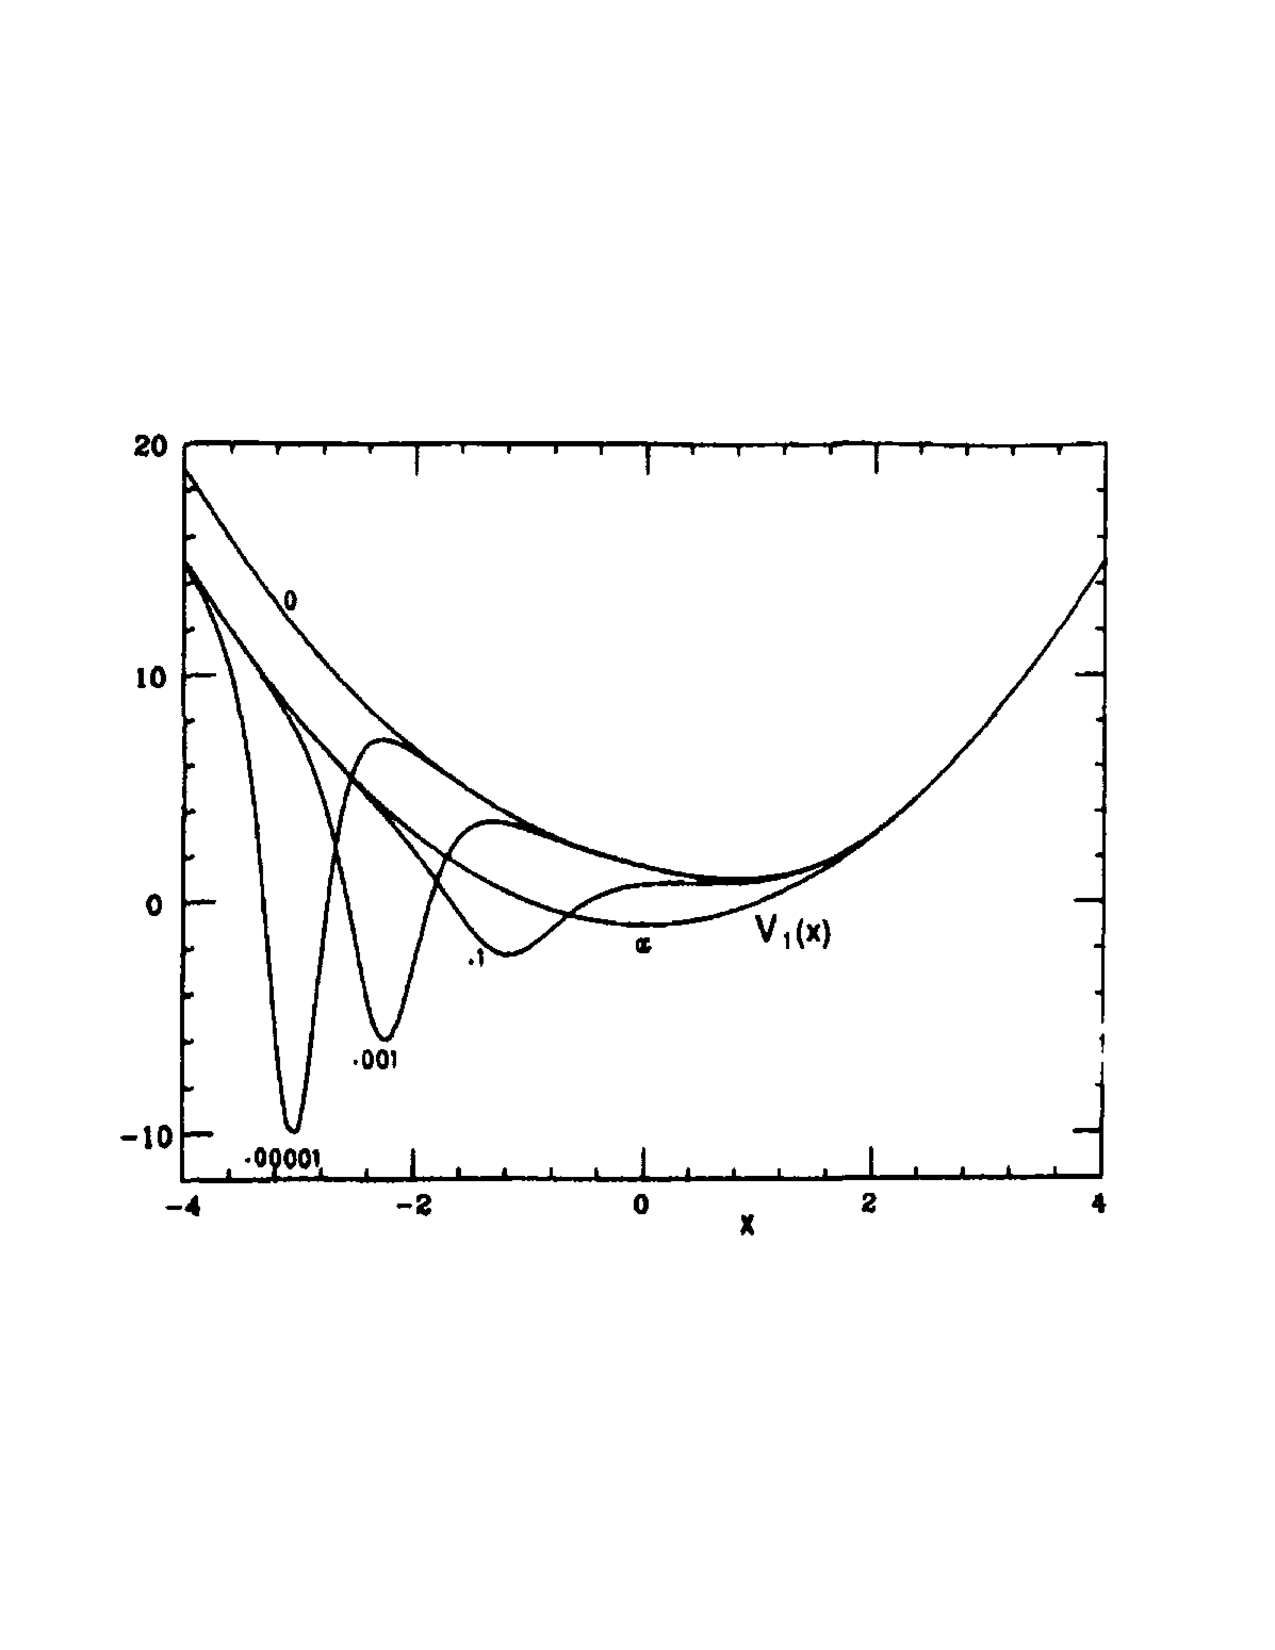
\includegraphics[height=8cm, keepaspectratio=1, trim=0cm 7cm 0cm 7cm]{pics/slika2}
	\caption{Potenciali $\tilde{V}^{(1)}$ za razli\v cne vrednosti $\lambda_1$. Izvorni $V^{(1)}$ je bil Harmonski
		oscilator, ki je tudi prikazan na grafu. Hamiltoniani s temi potenciali so popolnoma izospektralni.}
	\label{sl2}
\end{figure}

\begin{figure}[H]
	\centering
	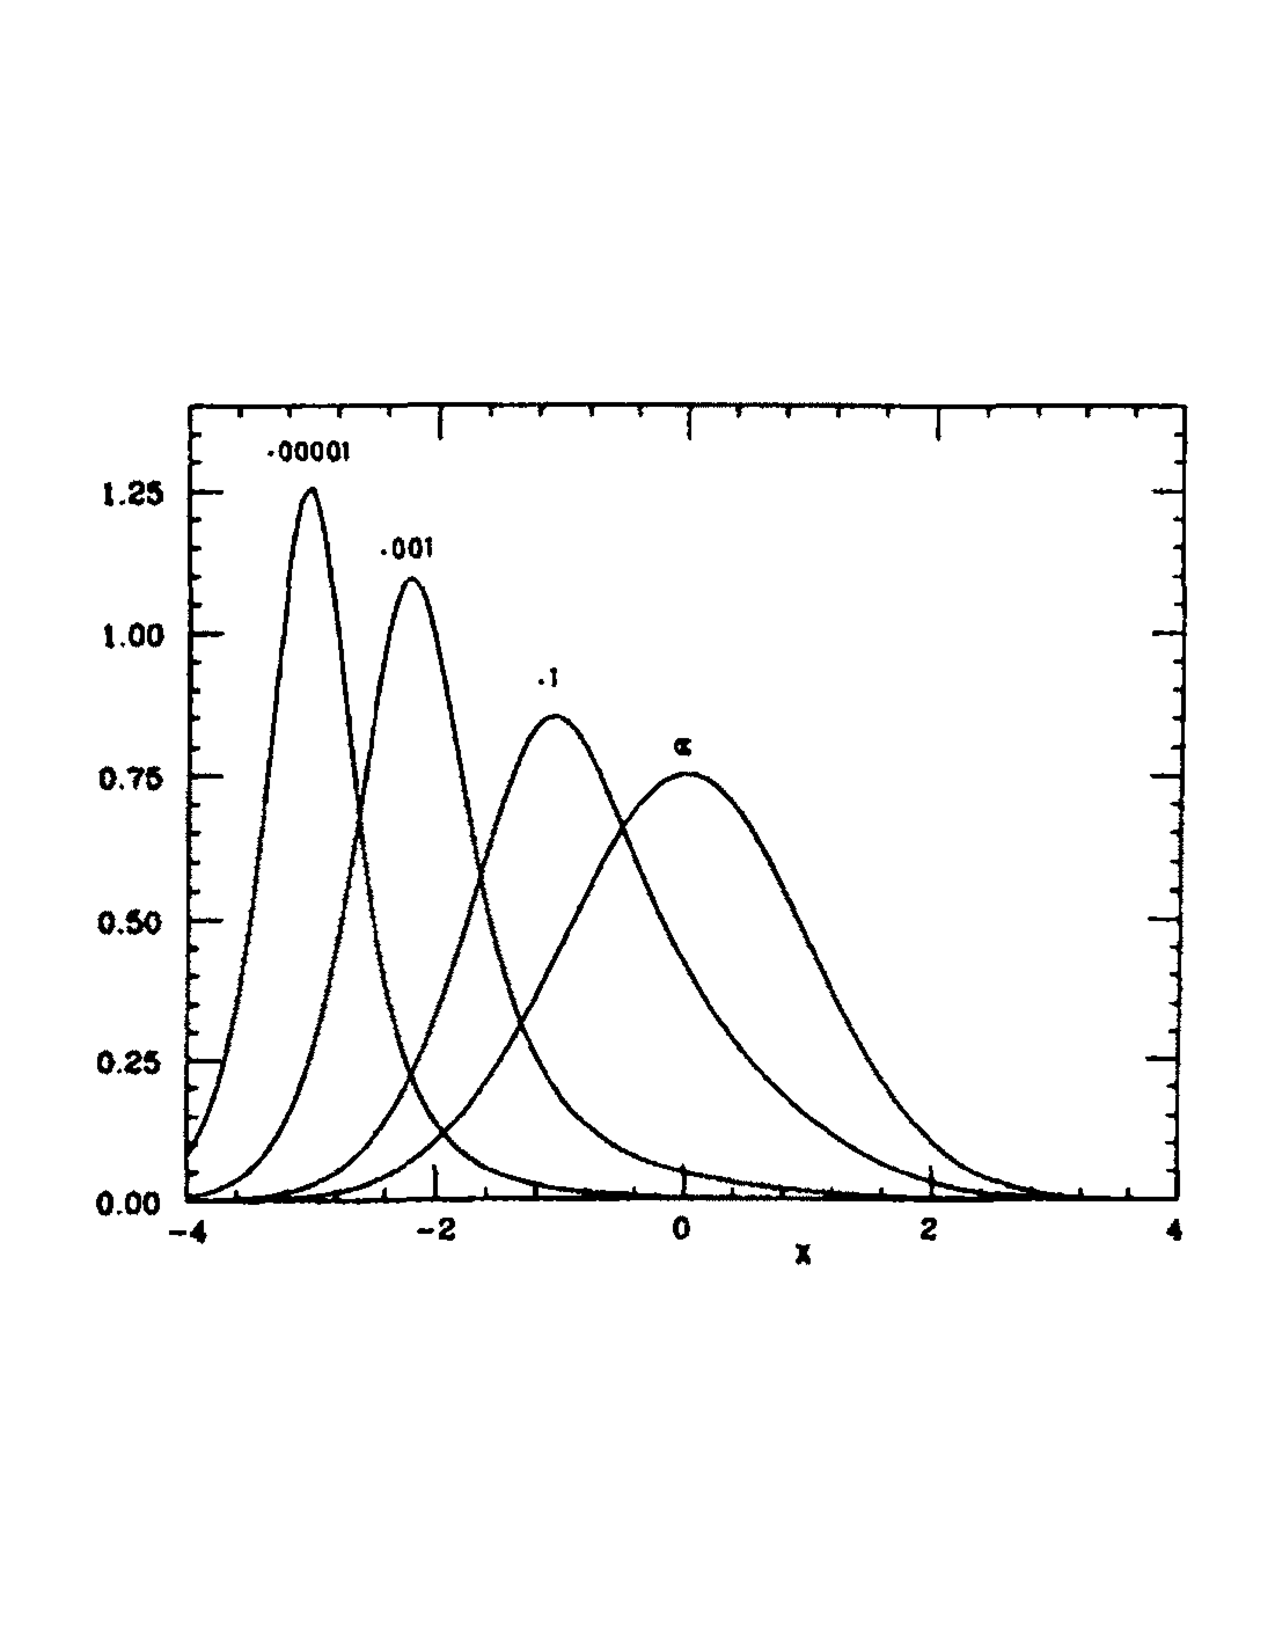
\includegraphics[height=8cm, keepaspectratio=1, trim=0cm 7cm 0cm 7cm]{pics/slika4}
	\caption{Graf prikazuje osnovne valovne funkcije k grafu iz slike~\ref{sl2}.}
	\label{sl3}
\end{figure}

Sedaj smo dobili dru\v zine potencialov, ki vrnejo vsa stanja ista, razen osnovnega, ki je odvisen od parametra $\lambda_1$.
Vendar gremo lahko korak dlje in isto naredimo za $V^{(2)}$, ki ga spremenimo v $\tilde{V}^{(2)}(x; \lambda_2)$, kar se potem
pomeni $V^{(1)} \to \tilde{V}^{(1)} (x; \lambda_1, \lambda_2)$. To lahko posplo\v simo na vsa vezana stanja in dobimo $\tilde{V}
^{(1)}(x; \underline{\lambda})$.

Taka dru\v zina potencialov, $\tilde{V}^{(1)}(x;\underline{\lambda})$, je popolnoma izospektralna, momente pa lahko nastavljamo
poljubno prek $\underline{\lambda}$.



\section{Supersimetrija v teoriji perturbacij}

Supersimetrija omogo\v ca dve novi perturbacijski metodi. Variacijska metoda je bolj intuitivna in tudi bistveno bolj
natan\v cna, ti. $\delta$-razvoj pa spominja na razvoj po zankah iz kvantne teorije polja, saj uporablja podobne prijeme
ki se uporabljajo pri regularizaciji interakcijskih \v clenov.

\subsection{Variacijski pristop}

Potencial $V_1$ ima \v clene, ki jih je treba obravnavati perturbativno. Za metodo potrebujemo testno valovno funckijo, $\psi_v$,
ki aproksimira osnovno stanje. Pri\v cakovana energija tega stanja bo na\v sa aproksimacija prave osnovne energije.
Upo\v stevamo en.~\eqref{riccati}.

\begin{equation}
	V_1(x) - E_0 = W^2(x) - \koren\px W(x).
\end{equation}

\ni s katero izra\v cunamo $W(x)$ do neke natan\v cnosti. Z njim lahko prek en.~\eqref{anihilator} in~\eqref{kreator} izra\v cunamo
operatorje dviganja, $a^\dagger$, in spu\v s\v canja, $a$, s katerima se lahko zavihtimo v vzbujena stanja.

Za\v cetno aproksimacijo $W(x)$ in $E_0$ dobimo prek variacijske metode, s testno funkcijo, ki aproksimira osnovno stanje. Po
navadi se jo aproksimira z Gaussovo krivuljo. Imejmo testno funkcijo $\psi_v (x;\eta)$, kjer parameter $\eta$ dolo\v cimo tako,
da minimizira energijo -- s tem dobimo aproksimacijo osnovnega stanja. Pri\v cakovana energija take testne valovne funkcije je

\begin{align}
	\langle E \rangle_\eta &= \langle \psi_v| H |\psi_v \rangle \notag \\
	&= \intinf\ \psi_v (x; \eta) H \psi_v (x; \eta) \notag \\
	&= \intinf\ \psi_v (x;\eta) \bigg[-\frac{1}{2}\px^2 + V_1(x)\bigg]\psi_v(x;\eta) \notag \\
	&= -\frac{1}{2}\intinf\ \psi_v(x;\eta)\ \px^2\ \psi_v (x;\eta) + \intinf\ \psi_v(x;\eta)V_1(x)\psi_v(x;\eta) \notag \\
	&= \intinf \bigg[\koren \px \psi_v(x;\eta)\bigg]^2 + \intinf\ \psi_v^2 (x; \eta) V_1 (x), \label{eeta}
\end{align}

\ni kjer smo v en.~\eqref{eeta} predpostavili, da je na\v sa testna funkcija integrabilna, analiti\v cna in da dovolj hitro pada, ko
$x \to \pm \infty$ -- ker je testna funkcija arbitrarna, lahko zadostimo vsem tem pogojem. Prav tako smo zgolj zaradi preprostosti
pisave predpostavili, da potencial $V_1$ komutira z falovno funkcijo, vendar to ni pravi pogoj.

Parameter $\eta$ dolo\v cimo tako, da minimizira energijo $\langle E \rangle_\eta$, tj. zahtevamo

\begin{equation}
	\frac{\partial \langle E \rangle_\eta}{\partial\eta}\bigg|_{\eta = \xi} = 0, \qquad
	\frac{\partial^2 \langle E \rangle_\eta}{\partial\eta^2}\bigg|_{\eta = \xi} > 0.
\end{equation}

\ni Energijo zato odvajamo po parametru $\eta$,

\begin{equation}
	\pe\langle E\rangle_\eta = \intinf\bigg[(\px \psi_v) \pe (\px \psi_v) +  2 \psi_v (\pe \psi_v) V_1\bigg].
\end{equation}

\ni Sedaj, ko imamo pribli\v zek za $E_0$ in $\psi_0$ lahko izra\v cunamo $W(x)$ prek identitete~\eqref{superpotencial}, tj.

\begin{equation}
	W (x; \xi) = -\koren\px\ln\psi_v (x;\xi),
\end{equation}

\ni s \v cimer dobimo par $V_1^\prime$ in $V_2^\prime$, ki sta pribli\v zka za $V_1$ in $V_2$. Potenciala $V_1^\prime$ in $V_2^\prime$
bi radi tak\v sna, da poznamo njuno to\v cno re\v sitev.

Ta metoda ima zelo veliko pomankljivost -- zelo dobro moramo uganiti $\psi_v$. Po navadi se uporablja ve\v c parametrov $\eta_i$, kjer
potem zahtevamo

\begin{equation}
	\partial_{\eta_i} \langle E \rangle_{\underline\eta}\Big|_{\underline{\eta} = \underline{\xi}} = 0, \ \forall \eta_i
\end{equation}

in pozitivnost determinante Hessejeve matrike glede na $n$-terec parametrov $\eta_i$ (pogoj za lokalni minimum).

\subsection{$\delta$-razvoj}

Razvoj po potencah $\delta$ nekoliko spominja na razvoj po zankah iz kvantne teorije polja. Metodo bom predstavil na konkretnem
primeru. Naj bo $V_1 (x) = 2gx^4$ anharmonski oscilator. Potenca $4$ je previsoka, re\v siti znamo samo za $x^2$, zato bomo
$V_1$ definirali kot analiti\v cno nadaljevanje harmonskega oscilatorja

\begin{equation}
	V_1 = 2gx^4 = M^{2 + \delta}x^{2 + 2\delta} - C(\delta) = W^2 - \koren\px W.
\end{equation}

\ni Parameter $M$ se je notri pri\v stulil tako kot pri dimenzijski regularizaciji iz kvantne teorije polja. Sicer je res, da delamo
z brezdimenzijskimi koli\v cinami, vendar ta skalirni faktor ostaja. Parameter $\delta$ nam predstavlja "`anharmonskost"' oscilatorja.
Energijo osnovnega stanja, $C(\delta)$ od\v stejemo za faktorizacijo hamiltoniana z operatorji $a$ in $a^\dagger$.

Pri $\delta = 0$ imamo $M = m$, pri kvarti\v cnem anharmonskem oscilatorju, $\delta = 1$, pa je $M = (2g)^{1/3}$. \v Ce sta $V_1$ in
$W$ analiti\v cna, potem za oba obstaja Taylorjev razvoj po potencah $\delta$,

\begin{equation}
	V_1 = M^2x^2\sum_{k = 0}^\infty \delta^k \frac{[\ln(Mx^2)]^k}{k!} - 2 \sum_{k = 0}^\infty \delta^k E_k,
	\label{delta-razvoj}
\end{equation}

\ni $E_k$ je energija osnovnega stanja potenciala $V_1$, ki je znan do reda $\delta^k$ nata\v cno. Analogno aproksimiramo tudi superpotencial
$W(x)$,

\begin{equation}
	W(x) = \sum_{k = 0}^\infty \delta^k W_{(k)}(x).
	\label{w-razvoj}
\end{equation}

Nadaljujemo tako, da na obeh straneh en.~\eqref{riccati} upo\v stevamo en.~\eqref{delta-razvoj} in~\eqref{w-razvoj}, ki mora veljati v
vseh redih razvoja -- dobimo sistem diferencialnih ena\v cb po redih $\delta^k$. V prvem redu dobimo harmonski oscilator

\begin{equation}
	W_{(0)}^2 - \px W_{(0)} = M^2x^2 - 2E_0,
	\label{diffena}
\end{equation}

\ni ki ima re\v sitve $W_{(0)} = Mx$ in $E_0 = M/2$. V drugem redu dobimo poleg en~\eqref{diffena} \v se ena\v cbo

\begin{equation}
	\px W_{(1)} - 2W_{(1)}W_{(0)} = - M^2x^2 \ln Mx^2 + 2E_1,
\end{equation}

\ni z re\v sitvami

\begin{equation}
	W_{(1)} = -\text{e}^{Mx^2} \int_0^x \d y\ \text{e}^{-My^2}\big[M^2y^2 \ln My^2 - 2E_1\big].
\end{equation}

Ta metoda je dobra, \v ce nimamo nobene predstave o problemu in si \v zelimo relativno grobo oceno osnovnega stanja. Za vzbujena stanja
je variacijska metoda natan\v cnej\v sa, vendar za visoka vzbujena stanja tudi ta podle\v ze vsled \v cesar moramo pose\v ci po
standarnih metodah.



\section{Zaklju\v cek}

Napredek v supersimetriji ima uporabo tudi v nerelativisti\v cni kvantni mehaniki.


\begin{thebibliography}{9}
	\bibitem{susyqm}
	F. Cooper, A. Khare in U. Sukhatme,
	\emph{Supersymmetry in Quantum Mechanics},
	World Scientific, 2001.
	\bibitem{introsus}
	P. West,
	\emph{Introduction to Supersymmetry and Supergravity},
	World Scientific, 1990.
	\bibitem{arxiv1}
	J. F. Cariñena in A. Ramos,
	\texttt{arXiv:math-ph/0311029v1},
	2003.
	\bibitem{arxiv2}
	J. F. Cariñena in J. de Lucas,
	\texttt{arXiv:0908.2235v1 [math-ph]},
	2009.
\end{thebibliography}

\end{document}
